\section{Current Scans}

\textbf{TODO: decide if this is necessary}

Occasionally during phase I, current scans were run. These consisted of running one beam at a series of beam currents, while the other beam was not running. An example of the change in current with time can be found in fig \ref{fig:CurrentEg}




\begin{figure}[htb]
	\centerfloat
		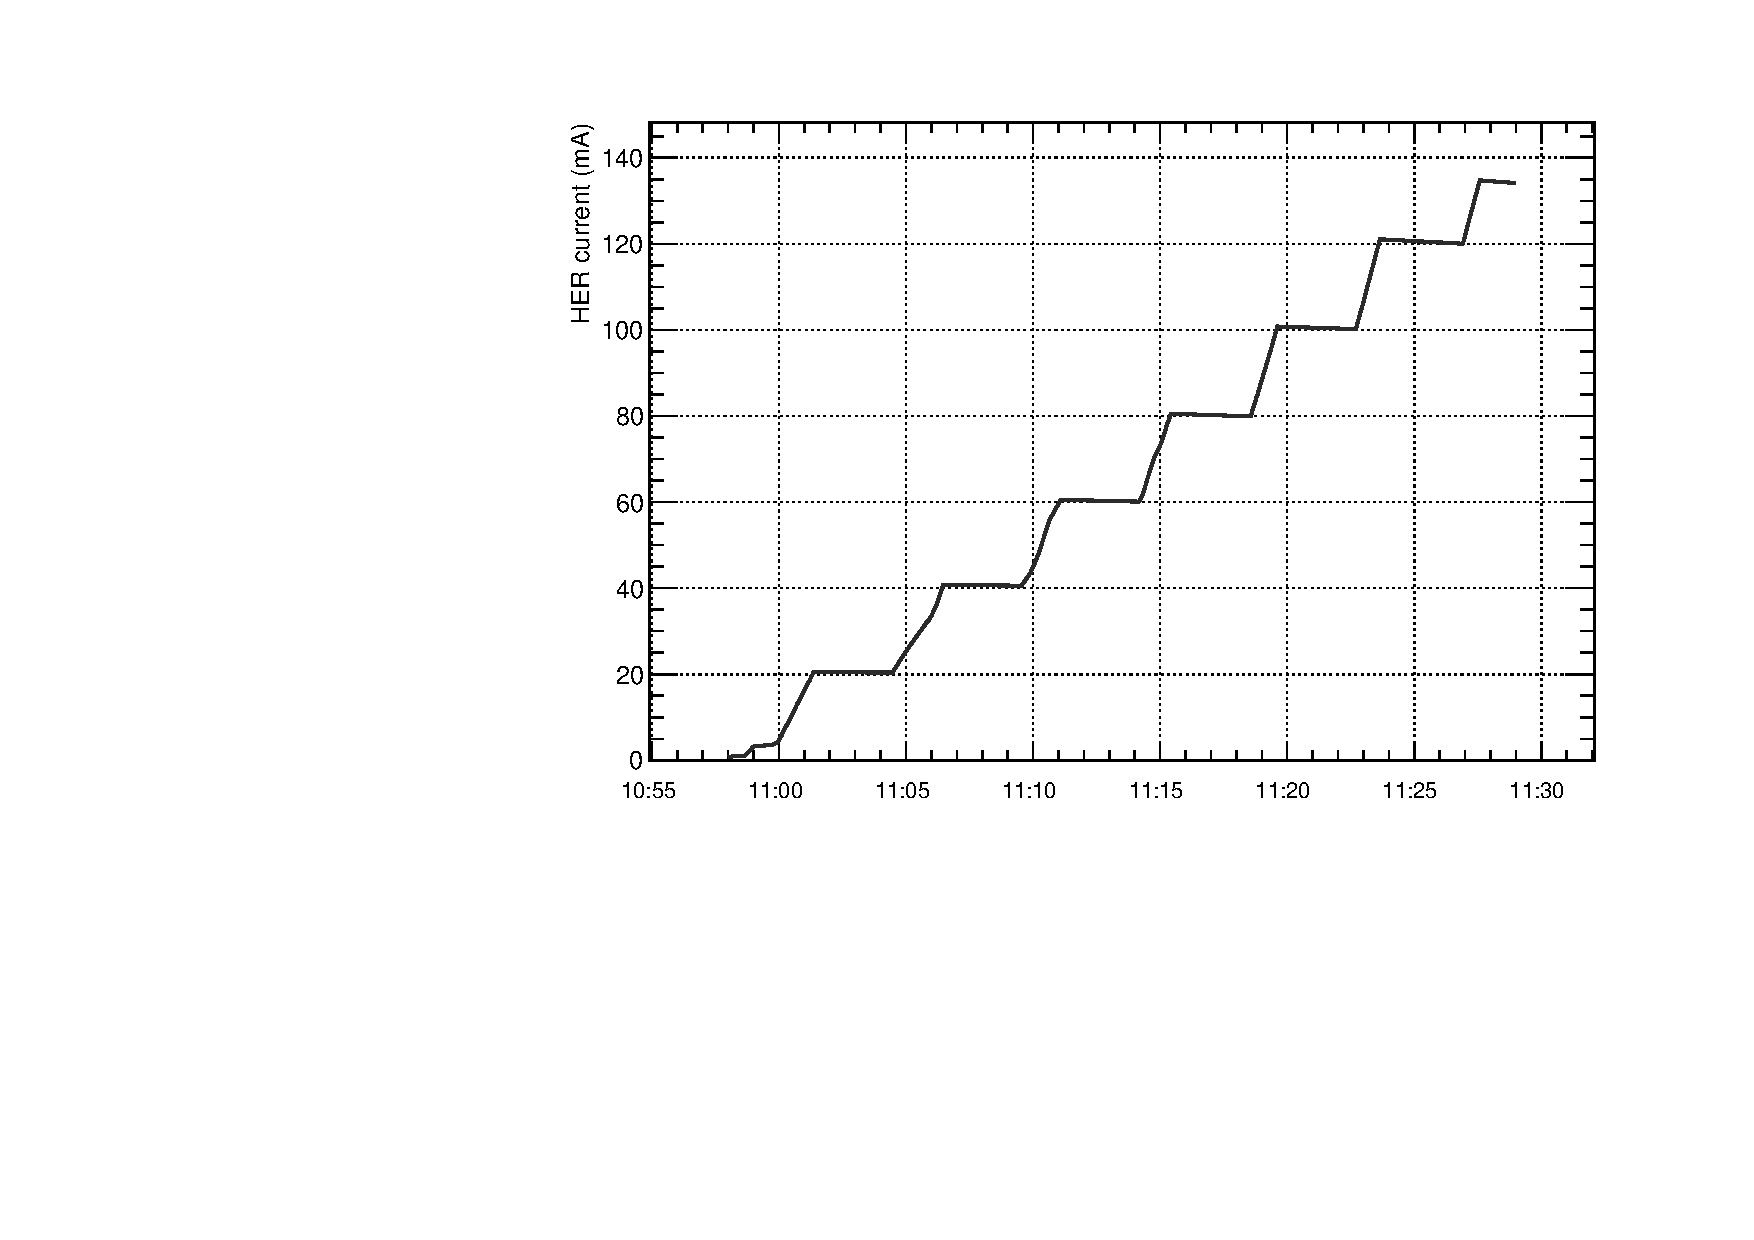
\includegraphics[trim={0 0 0 0.75cm},clip, width=\textwidth]{images/CurrentScan}
	\caption{Example of beam current change during current scan}	
	\label{fig:CurrentEg}
\end{figure}



\section{Beam Current Scans}

\textbf{TODO: Determine if this is worth showing. Show current vs rate for both beams, and also for real and sim. Compare response (linear, quadratic)}


\begin{figure}
	\centering
	\subfigure[Data]{
		\begin{overpic}[width=\textwidth]{images/LERCurrentFill}
		\end{overpic}
		\label{fig:LERCurScanData}
	}
	\subfigure[Simulation]{
		\begin{overpic}[width=\textwidth]{images/LERCurrentFill_sim}
		\end{overpic}
		\label{fig:LERCurScanSim}
	}
	\caption[LER Current Scan]{LER Current Scan}		
\label{fig:LERCURScan}
\end{figure}

\begin{figure}
	\centering
	\subfigure[Data]{
		\begin{overpic}[width=\textwidth]{images/HERCurrentFill}
		\end{overpic}
		\label{fig:HERCurScanData}
	}
	\subfigure[Simulation]{
		\begin{overpic}[width=\textwidth]{images/HERCurrentFill_sim}
		\end{overpic}
		\label{fig:HERCurScanSim}
	}
	\caption[HER Current Scan]{HER Current Scan}		
\label{fig:HERCURScan}
\end{figure}


\section{Touschek Experiments}


Fig \ref{fig:TousRatio} shows the Touschek ratio, and fig \ref{fig:BGasRatio} shows the beam-gas ratio.




Using the analysis technique described in \ref{sec:PBump}, it was determined that Z=2.7 for the LER. The number of bunches in the ring is omitted, as it is constant during the experiment. $c_{gas}$ will then be the beam-gas component of the rate, and $c_{T}$ will be the beam-beam component of the rate. Figure \ref{fig:beamSizeScan} shows the result of this fit for several beam size scan runs. The fit values of $c_{gas}$ and $c_{T}$ can be found in fig \ref{fig:LERSimCompare}.

	The same procedure was applied to simulated data as well, and the results are also included in fig \ref{fig:LERSimCompare}. The simulation was done assuming Z=7 (see Chapter \ref{chap:Sim}), so this value was used in Eqn \ref{eqn:TousFit} instead of Z=2.7.

	In order to verify the accuracy of the simulation, a ratio of the data to simulation for the Touschek and beam-gas parameters is defined:
\begin{subequations}
\begin{align}
		{R_{gas} = c_{gas}^{data}/c_{gas}^{sim}} \\
		{R_{T} = c_{T}^{data}/c_{T}^{sim}}
\end{align}
\end{subequations}
The more accurate the simulation is, the closer these ratios will be to 1. These ratios can also be used to scale simulation to better match the data. Fig \ref{fig:TousRatio} shows the Touschek ratio, and fig \ref{fig:BGasRatio} shows the beam-gas ratio.




\begin{figure}
	\centering
	\subfigure[Touschek]{
		\begin{overpic}[trim={0 0 0 0.75cm},clip, width=\textwidth]{images/TouschekFit}
		\end{overpic}
		\label{fig:LERTousRes}
	}
	\subfigure[Beam-Gas]{
		\begin{overpic}[trim={0 0 0 0.75cm},clip, width=\textwidth]{images/BeamGasFit}
		\end{overpic}
		\label{fig:LERBGasRes}
	}
	\caption[Touschek and beam-gas fit parameters]{Touschek and beam-gas fit parameters. Bars are simulation, points are data. Red is HER, and blue is LER}
\label{fig:LERSimCompare}
\end{figure}






\begin{figure}
	\centering
	\subfigure{
		\begin{overpic}[width=\textwidth]{images/TouschekRatioPlot}
		\end{overpic}
		\label{fig:TousRatio}
	}
	\subfigure{
		\begin{overpic}[width=\textwidth]{images/BeamGasRatioPlot}
		\end{overpic}
		\label{fig:BGasRatio}
	}
	\caption[Ratio of data to simulation]{Ratio of data to simulation. Blue is the LER, red is the HER}
\label{fig:DataSimRatio}
\end{figure}





\begin{table}
	\centering
	\begin{tabular}{ lcccc }
			&	\multicolumn{2}{c}{HER}			& \multicolumn{2}{c}{LER}			\\
  			&  Beam-gas  		& Beam-beam		&  Beam-gas 		& Beam-beam  		\\ 
	Channel ($\phi$)&  [$Hz/(mA\cdot Pa)$]	& [$Hz\cdot\mu m/mA^{2}$]	& [$Hz/(mA\cdot Pa)$]	& [$Hz\cdot\mu m/mA^{2}$]\\ \hline \hline
	0 (0$^{\circ}$) & 32800$\pm$700	& 1.48$\pm$0.29$\times10^{-4}$	& 7520$\pm$110		& 9.8$\pm$0.8$\times10^{-3}$			\\	
	1 (90$^{\circ}$)& 15700$\pm$500	& 0.39$\pm$0.19$\times10^{-4}$	& 3880$\pm$70		& 4.9$\pm$0.5$\times10^{-3}$			\\
	2 (180$^{\circ}$)& 24500$\pm$600& 1.13$\pm$0.25$\times10^{-4}$	& 6650$\pm$90		& 8.0$\pm$0.7$\times10^{-3}$			\\
	3 (270$^{\circ}$)& 32400$\pm$700& 1.71$\pm$0.29$\times10^{-4}$	& 9340$\pm$10		& 10.8$\pm$0.8$\times10^{-3}$			\\ \hline

	\end{tabular}
	\caption[Beam-beam fits]{\textbf{TODO: Better way to present this?}}
	\label{tab:beam beam fits}
\end{table}









\begin{figure}
	\centerfloat
		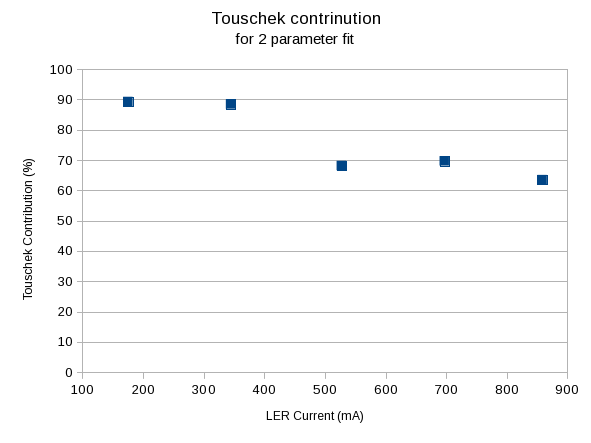
\includegraphics[width=\textwidth]{images/touschekPercent}
	\caption{Touschek contribution vs LER current for a beam size of 90$\mu m$}	
	\label{fig:TouschekContribLER}
\end{figure}


